
\section{System define and problem formulation}
\label{sec:systemmodel}
 
\subsection{Ground-to-Air Communication Model}

We consider a set of ground nodes (GNs) denoted by $\mathcal{N} = \{1, 2, \dots, n\}$, distributed along a pre-defined flight mission path,  such as bridges and railways, water, gas, and oil pipelines, and rivers and coastlines. 
Each  $GN_i \ ,\ i\in \mathcal{N}$ is located at a fixed position and has a specific volume of data to be collected by the UAV.
The smaller the index of the $GN$ means closer to the start point of the flight path.

Following the practical ground-to-air communication model established in~\cite{CommunicationModel}, the communication range of a $GN$ is determined by the two-dimensional distance between the $GN$ and the UAV. 
Let $(r_{i},h_{i})$ denote the relative horizontal and vertical distance of UAV from certain ground node $GN_i$.
The UAV can establish a reliable communication link with $GN_i$ only when the path loss caused by the distance between them $PL_i(r_i,h_i)$ is within threshold $PL^{max}_i$.
Specifically, the condition for data transmission is given by:
$$PL_i(r_i,h_i) \leq PL^{max}_i, $$ 
where the threshold $PL^{max}_i$ of certain $GN_i$ is determined by the ground node itself and given in advancing. 
The connection between UAV and the GN would loss, when the path loss exceeds $PL^{max}_i$ for $GN_i$. 

\begin{multline}
    PL_i(r_i,h_i)
    =\frac{\mu_{LoS}-\mu_{NLoS}}
    {1+a \exp(-b[\frac{180}{\pi}\arctan(\frac{h_{i}}{r_{i}})-a])} \\
    +10 \log(h_{i}^2+r_{i}^2)+M
    \label{equ:PL}
\end{multline}

Eq.~(\ref{equ:PL}) gives the expected path loss under the probabilistic line-of-sight (LoS) model~\cite{CommunicationModel}, where $\mu_{LoS}$ and $\mu_{NLoS}$ are the mean excess losses of LoS and non-LoS links, and $a$ and $b$ are environment-dependent parameters.
The constant $M$ collects the carrier-frequency and free-space propagation factors together with the NLoS excess loss:
\begin{equation}
    M=20\log f+20\log\left(\frac{4\pi}{c}\right)+\mu_{NLoS},
    \label{equ:M}
\end{equation}
where $f$ is the carrier frequency and $c$ is the speed of light.

The key angular variable is the link elevation angle $\theta_i=\frac{180}{\pi}\arctan(h_i/r_i)$ (in degrees), measured between the GN--UAV line and the horizontal plane.
It determines the LoS probability $P_{LoS}(\theta_i)=1/(1+a\exp(-b[\theta_i-a]))$: a larger $\theta_i$ increases the LoS probability and thus reduces the expected excess loss when $\mu_{LoS}<\mu_{NLoS}$.
However, at a fixed horizontal distance, increasing altitude also lengthens the slant range $d_i=\sqrt{h_i^2+r_i^2}$ and increases the free-space loss.
These competing effects determine the altitude-dependent communication region defined by $PL_i(r_i,h_i)\leq PL_i^{max}$, as illustrated in Fig.~(\ref{fig:communication_range}).

To model the data upload, we characterize each $GN_i$ by a nominal SINR $\gamma_i$, which is a per-node design parameter given in advance---like the path-loss threshold $PL_i^{max}$---rather than the instantaneous, position-dependent SINR experienced by the UAV. Letting $B$ denote the channel bandwidth, the achievable rate of the link is evaluated at this nominal SINR through the Shannon capacity:
\begin{equation}
    \bar{R}_i = B\log_2(1+\gamma_i). \label{equ:const_rate}
\end{equation}
Each $GN_i$ therefore uploads data at the constant rate $\bar{R}_i$ throughout the collection phase, which yields the deterministic collection duration $\tau_i = D_i/\bar{R}_i$.

\begin{figure}[]
  \centering
   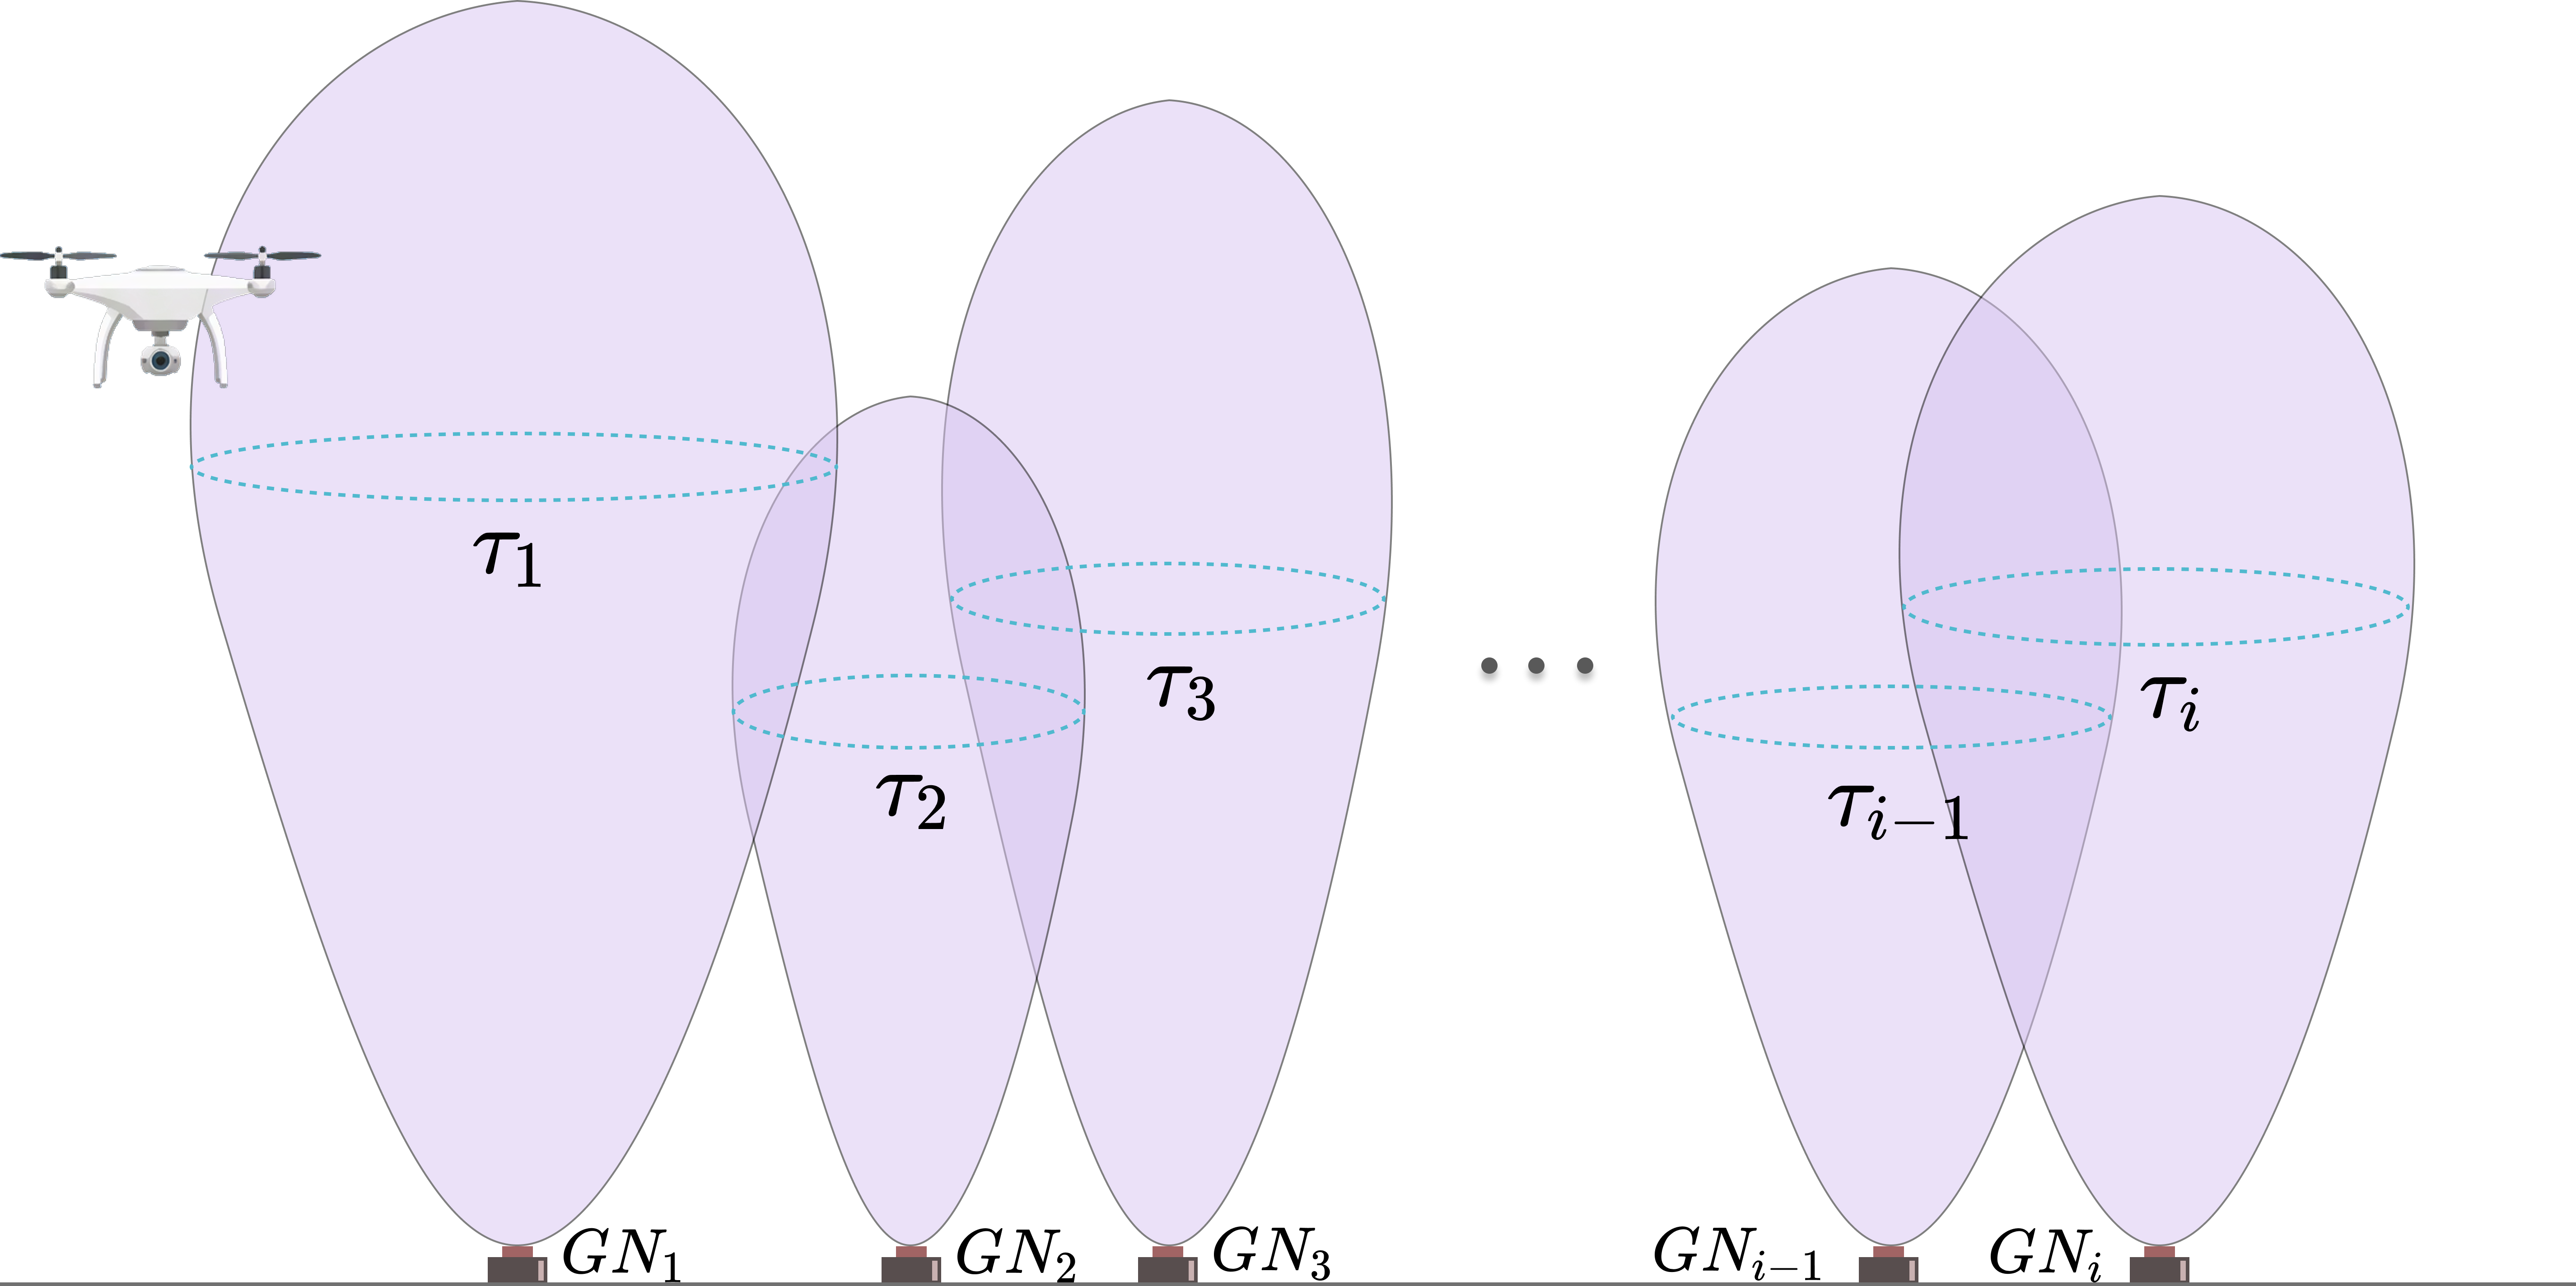
\includegraphics[width = 1\linewidth]{figures/gn-communication-range-3d.png}
    \caption{Altitude-dependent communication regions defined by Eq.~(\ref{equ:PL}) and Eq.~(\ref{equ:M}).
    The UAV must remain within the region of $GN_i$ for the required data collection duration $\tau_i = D_i/\bar{R}_i$, where $D_i$ is the data volume of $GN_i$ and $\bar{R}_i = B\log_2(1+\gamma_i)$ is the constant achievable rate.}\label{fig:communication_range}
\end{figure}

The link elevation angle differs from the UAV's flight-path angle, which describes the direction of its velocity.
Horizontal and vertical speed decisions change $r_i$ and $h_i$ over time, thereby changing both $\theta_i$ and $d_i$ and determining how long the UAV remains within each GN's communication region.
This geometric dependence couples speed and altitude scheduling with the required data collection duration.

\subsection{Flight Energy Consumption Model}

To optimize the UAV's horizontal and vertical speeds for energy-efficient data collection, we first model its propulsion power as a function of these two velocity components.
Following~\cite{GongHao}, we express the total power as the hovering power plus the increments associated with horizontal and vertical motion.

\begin{figure}[]
  \centering
   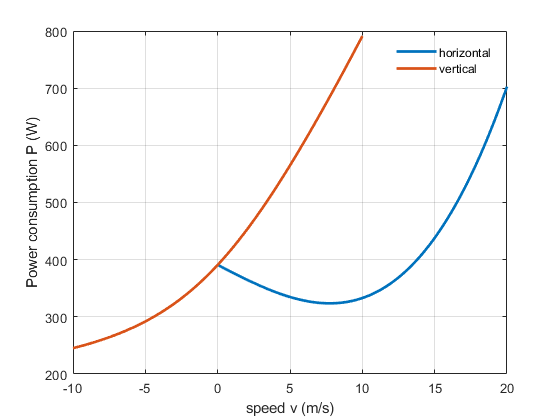
\includegraphics[width = 0.8\linewidth]{figures/uav-power-vs-velocity.png}
    \caption{Horizontal and vertical propulsion power functions used in the simulations.
    The horizontal power in Eq.~(\ref{equ:h_2}), modeled by a cubic polynomial fitted to flight-test measurements, initially decreases and then increases with horizontal speed, reaching a minimum at an intermediate speed.
    The vertical power in Eq.~(\ref{equ:v_1}) increases monotonically with the climb rate.
    Both functions yield the same hovering power, $P_{mh} = 390.95\,\mathrm{W}$, at zero speed.}
\end{figure}

Let $V_{total}$ denote the total (resultant) flight speed and $\gamma$ the flight pitch angle, defined as the angle between the velocity vector and the horizontal plane. The horizontal and vertical velocity components are related to $V_{total}$ and $\gamma$ by
\[
    V_{\parallel} = V_{total}\cos\gamma, \qquad V_{\perp} = V_{total}\sin\gamma.
\]

\begin{equation}
    P_{total}(V_{total}) = P_{mh} + \Delta P_{\parallel}(V_{\parallel}) + \Delta P_{\perp}(V_{\perp}),
    \label{equ:e_1}
\end{equation}

In Eq.~(\ref{equ:e_1}), $P_{mh}$ denotes the hovering power, while $\Delta P_{\parallel}(V_{\parallel})$ and $\Delta P_{\perp}(V_{\perp})$ denote the power increments associated with horizontal and vertical motion, respectively.
This additive model evaluates the two contributions separately to obtain the instantaneous propulsion power during three-dimensional flight.

\textbf{For the horizontal component}, we adopt the analytical propulsion power model in~\cite{GongHao}:

\begin{align}
    &P_{\parallel} = P_{mh}+ \frac{3}{8}\sqrt{n}\delta\sqrt{\frac{W\rho A}{C_{T}}}s||V_{\parallel}||^2+P_{in}
    \nonumber
    \\ &\left[\left(\sqrt{1+\frac{||V_{\parallel}||^4}{4v_0^4}}-\frac{||V_{\parallel}||^2}{2v_0^2}\right)^{1/2}-1\right]+\frac{n}{2}S_{FP\parallel \cdot \rho} ||V_{\parallel}||^3
    \label{equ:h_1}
\end{align}

$$P_{in}\triangleq 1.11 \frac{W^{3/2}}{\sqrt{2n\rho A}}$$

Here, $W$ is the UAV weight, $n$ is the number of rotors, $\rho$ is the air density, and $A$ is the rotor disc area.
The parameters $\delta$, $s$, $C_T$, and $S_{FP\parallel}$ denote the profile drag coefficient, rotor solidity, thrust coefficient, and equivalent flat-plate area, respectively, while $v_0$ is the mean induced velocity in hover.

To simplify platform-specific calibration and numerical evaluation, we use a cubic approximation in the simulations:

\begin{equation}
    P_{\parallel} = c_1 v_{\parallel}^3 + c_2 v_{\parallel}^2 + c_3 v_{\parallel} + P_{mh}\label{equ:h_2}
\end{equation}

The coefficients $c_1$, $c_2$, and $c_3$ are fitted to the flight-test measurements reported in~\cite{assume}, with their values given in Section~\ref{sec:simulation}.
The constant term $P_{mh}$ ensures that both models yield the same power at zero speed.
The fitted model captures the decrease and subsequent increase of horizontal power with speed, and its convexity over the operating range is established below.

\textbf{For the vertical component}, we adopt the steady-state propulsion power model in~\cite{PowerConsumptionModel}.
Under constant-speed vertical flight, rotor thrust balances the UAV weight, and the required power comprises a velocity-dependent induced term and a constant blade-profile term:

\begin{equation}
    P_{\perp} = k_1 mg \left[\frac{V_{\perp}}{2}+\sqrt{\left(\frac{V_{\perp}}{2}\right)^2+\frac{mg}{k_2^2}}\right] + c_1(mg)^{3/2}
    \label{equ:v_1}
\end{equation}

Here, $V_{\perp}$ is the vertical velocity, $m$ is the UAV mass, and $g$ is the gravitational acceleration.
The coefficient $k_1$ corrects for non-uniform rotor inflow, $k_2$ characterizes the induced-flow contribution, and $c_1$ accounts for blade-profile power.
The first term describes the power required to generate thrust, while $c_1(mg)^{3/2}$ represents the power needed to overcome blade drag.
Parasite power is neglected at the moderate vertical speeds considered here.

The parameters $k_1$ and $c_1$ are adopted from~\cite{PowerConsumptionModel}, while $k_2$ and $mg$ are calibrated to approximately match the horizontal model's hovering power, with their values given in Section~\ref{sec:simulation}.

\begin{lemma}[Convexity of the vertical power component]
    \label{lem:ver}
    For any platform parameters $k_1 > 0$, $k_2 > 0$, $c_1 \geq 0$ and weight $mg > 0$, the vertical power function Eq.~(\ref{equ:v_1}) is strictly convex.
\end{lemma}

\begin{proof}
    See Appendix~\ref{pro:Lemma ver} \qed
\end{proof}

\begin{lemma}[Convexity of the horizontal power component]
    \label{lem:hor}
     Write Eq.~(\ref{equ:h_1}) as $P_\parallel(v) = c_1v^3 + c_2v^2 + P_{in}\cdot f(v) + P_{mh}$, where $c_1$ and $c_2$ denote the (positive) coefficients of the parasite terms and blade-profile, $P_{in} > 0$ is the induced-power constant, and $f(v) = [\sqrt{(1 + (v^2/2v_0^2)^2)} - v^2/2v_0^2]^{1/2} - 1$ is the induced-power increment with the mean hover induced velocity $v_0 > 0$.
     Then Eq.~(\ref{equ:h_1}) is strictly convex on $v \geq 0$ whenever $4c_2v_0^2 > P_{in}$, a condition satisfied by conventional multi-rotor configurations, including the platform parameters reported in~\cite{GongHao}.
\end{lemma}

\begin{proof}
    See Appendix~\ref{pro:Lemma hor} \qed
\end{proof}

The strict convexity of the two power components supports the constant-speed optimality results developed in Section~\ref{sec:problemanalysis}.
For the polynomial model in Eq.~(\ref{equ:h_2}), this property can be assessed through its second derivative, $P_\parallel''(v)=6c_1v+2c_2$.
With the parameter values used in Section~\ref{sec:simulation}, this derivative remains positive over the operating speed range, allowing the fitted model to retain the convexity required by the analysis.
For other UAV platforms, the applicability of these results should be assessed using the corresponding model parameters and operating range, together with the remaining assumptions of the formulation.


\subsection{Problem Definition}
\label{subsection:problem}

Let the UAV trajectory be denoted by $q(t) = (d(t), h(t))$, where $d(t)$ and $h(t)$ are the horizontal position along the mission path and the flight altitude at time t, respectively, and let $v_\parallel(t) = \dot{d}(t)$ and $v_\perp(t) = \dot{h}(t)$ be the corresponding velocity components.
Let $v_\parallel \in [0, V_{\parallel}^{max}]$, $|v_\perp| \leq V_{\perp}^{max}$ be the speed limits imposed by hardwares.
By Eq.~(\ref{equ:PL}), each $GN_i$ is associated with an altitude-dependent communication region in the $(d, h)$ plane, obtained from $PL(r_i, h_i) = PL_{max}^i$; we say that the UAV is inside the region of $GN_i$ at time $t$ if $(d(t), h(t))$ satisfies the corresponding path-loss condition.
The total flight energy follows directly from the decoupled flight energy consumption model Eq.~(\ref{equ:e_1}):
\begin{equation}
     E_{total}(q(\cdot)) = \int_0 ^T [P_{mh} + \Delta P_\parallel(v_\parallel(t)) + \Delta P_\perp(v_\perp(t))] dt 
\label{equ:Etotoal}
\end{equation}
where $T$ is the total mission time.

\begin{definition}[JHVSO problem]\label{def:JHVSO}
    Given ordered ground nodes $GN_1,\ldots,GN_N$, their communication regions, and the data volume $D_i$ of each $GN_i$, the \textit{JHVSO} problem seeks a trajectory $q(t)=(d(t),h(t))$ and collection intervals that minimize the total flight energy in Eq.~(\ref{equ:Etotoal}).
    Under the constant achievable rate $\bar{R}_i$ in Eq.~(\ref{equ:const_rate}), collecting the data volume $D_i$ requires a duration $\tau_i = D_i/\bar{R}_i$; the collection of $GN_i$ is successful if and only if the UAV stays within its communication region for a total duration of at least $\tau_i$.
    The UAV must serve the nodes in order, collecting from one node at a time, and fly from the prescribed initial position at altitude $h_0$ to a point within the last node's communication region and an altitude of $h_f$.
    The flight altitude is additionally bounded by $h_{\min} \le h(t) \le h_{\max}$, where $h_{\min}$ and $h_{\max}$ are the lower and upper altitude limits.
\end{definition}

The starting altitude $h_{0}$ and final altitude $h_f$ are exogenous mission parameters specified per scenario.
%%%%%%%%%%%%%%%%%%%%%%%%%%%%%%%%%%%%%%%%%%%%%%%%%%%%%%%%%%%%%%%%%%%%%%%%%%%%%%%%%%
%%%%%%%%%%%%%%%%%%%%%%%%%%%%%%%%%%%%%%%%%%%%%%%%%%%%%%%%%%%%%%%%%%%%%%%%%%%%%%%%%%
